\documentclass[portrait, a0paper, margin=.5cm]{baposter}

\usepackage{poster_style}

\begin{document}
    \begin{poster}%
    {
        grid=false,
        eyecatcher=true,
        bgColorOne=white,
        bgColorTwo=white,
        borderColor=IGNGrey,
        headerColorOne=IGNGrey,
        headerColorTwo=IGNGrey,
        headerFontColor=white,
        boxColorOne=white,
        boxColorTwo=white,
        colspacing=.5em,
        columns=6,
        textborder=rounded,
        headerborder=closed,
        headerheight=0.12\textheight,
        headershape=rounded,
        textfont={\color{IGNDarkGrey}},
        boxshade=plain,
        background=none,
        linewidth=1pt
    }
    {}
    {
        \color{IGNDarkGrey}
        3D Building model semantic evaluation
    }
    {
        \small
        \vspace{.5cm}
        \begin{tabular}[t]{c@{\extracolsep{4em}}c@{\extracolsep{4em}}c@{\extracolsep{4em}}c}
            Oussama Ennafii${}^1$ & Arnaud Le Bris${}^1$ & Florent Lafarge${}^2$ & Clément Mallet${}^1$ \\
        \end{tabular}
        {}\\
~\\
        ${}^1$        Univ. Paris-Est, LaSTIG MATIS, IGN, ENSG, 94160 Saint-Mandé, France\\
        ${}^2$        Inria, Titane, 06902 Sophia Antipolis, France
        {}\\
~\\
        \small oussama.ennafii@ign.fr
    }
    {
        \begin{tabular}{c}
            
\includegraphics[width=2.2cm]{theme/ign_logo}\\~\\
            
\includegraphics[width=2.2cm]{theme/paris_est_logo}
        \end{tabular}
    }

        \TransitionBox{motivation}{}{{\large \sc Motivation:} Why do we need automatic scene evaluation?}

        \StandardBox{context}{column=0, span=3, row=.03}{Context}{
            \begin{itemize}[label=, leftmargin=*]
                \item Urban models have a wide application range~\cite{Biljecki2015} (\textit{c.f.} next Table);
                \item Automatic urban modeling is an active research area~\cite{Musialski2012}, but {\color{IGNGreen}not yet operational};
                \item \textbf{Example:} The IGN solution, $\text{Bati3D}^\text{\textregistered}$, requires a considerable time to manually correct buildings.
            \end{itemize}
        }

        \StandardBox{applications}{column=3, span=3, aligned=context, bottomaligned=context}{Urban models applications}{
        \begin{center}
            \begin{tabular}{l l l}
                \toprule
                Planning & Simulation & Visualization \\
                \midrule
                City planning & Micro climates & Architecture \\
                Emergency intervention & Wave propagation & Cadastre \\
                Home decoration & Run-off water & Tourism \\
                Communication network & Military intervention & Video games \\
                \bottomrule
            \end{tabular}
        \end{center}
        }

        \StandardBox{auto_evaluation}{column=0, span=2, below=context}{Self Diagnostic}{
        Can be used for:
        \begin{itemize}[label=--, leftmargin=1.5em]
            \item Change detection;
            \item Urban models correction;
            \item Urban reconstruction method evaluation;
            \item Crowd reconstruction quality assessment.
        \end{itemize}
        }
        \StandardBox{state_art}{column=2, span=4, aligned=auto_evaluation, bottomaligned=auto_evaluation}{State of the art}{
            Urban models quality assessment methods can be divided as follows:
            \begin{itemize}[label=--, leftmargin=1em]
                \item Methods that gives {\color{IGNGreen} geometric indices} (for instance, heigh accuracy, completness \dots) by comparing to a {\color{IGNGreen} higher precision model}~\cite{Voegtle2003, Henricsson1997}.
                \item Methods that outputs end user oriented {\color{IGNGreen} topological and geometric errors} using {\color{IGNGreen}remote sensing data} (LiDAR, DSM, Orthoimage)~\cite{boudet2006supervised, Michelin2013}.
            \end{itemize}
        }

        \TransitionBox{formul}{below=auto_evaluation}{{\large \sc Problem formulation:} We want to build the least reference dependent possible automatic method for urban model diagnostic.}


        \StandardBox{taxonomy}{column=0, span=4, row=.315}{Error taxonomy}{
            \includestandalone[mode=buildnew, width=\textwidth]{mind_map}
~\\
            \textbf{Definitions}\\
~\\
            \begin{tabular}{x{2em} l c l}
                & \textbf{finesse} & : & error semantization level $\equiv$ depth in the taxonomy mind map.\\
                & \textbf{exclusivity} & : & error family hierarchization.
            \end{tabular}
        }

        \StandardBox{feats}{column=4, span=2, aligned=taxonomy}{Features}
        {
            We define a baseline for:
            \begin{enumerate}[label = (\roman*)., font=\color{black}, itemsep=15pt]
                \item Basic intrinsic descriptors:
                \begin{itemize}[label=$\blacktriangleright$, font=\color{IGNGreen}]
                    \item \textbf{Geometric} features based on the graph $\mathscr{G}=(facets, E)$\footnote{$E \triangleq \{(f, g) \in facets \times facets: \text{f and g are adjacent}\}$};
                \end{itemize}
                \item Optional descriptors:
                \begin{itemize}[label=$\blacktriangleright$, font=\color{blue}, itemsep=10pt]
                    \item \textbf{Altimetric} features based on the residual of the model height profile and the correponding DSM\@;
                    \item \textbf{Radiometric} features based on building wise normalized histograms of angle correlation\footnote{$C_I(s) \triangleq \{ \frac{\nabla I(p) . \vec{n}(s)}{\vert\nabla I(p)\vert}: p \in I \text{ and } p \cap s \neq \emptyset \}$} between gradients and footprint segments;
                \end{itemize}
            \end{enumerate}
        }

        \StandardBox{errors}{column=0, span=4, below=taxonomy}{Error samples}{
            \begin{multicols}{4}
                \begin{center}
                    \fbox{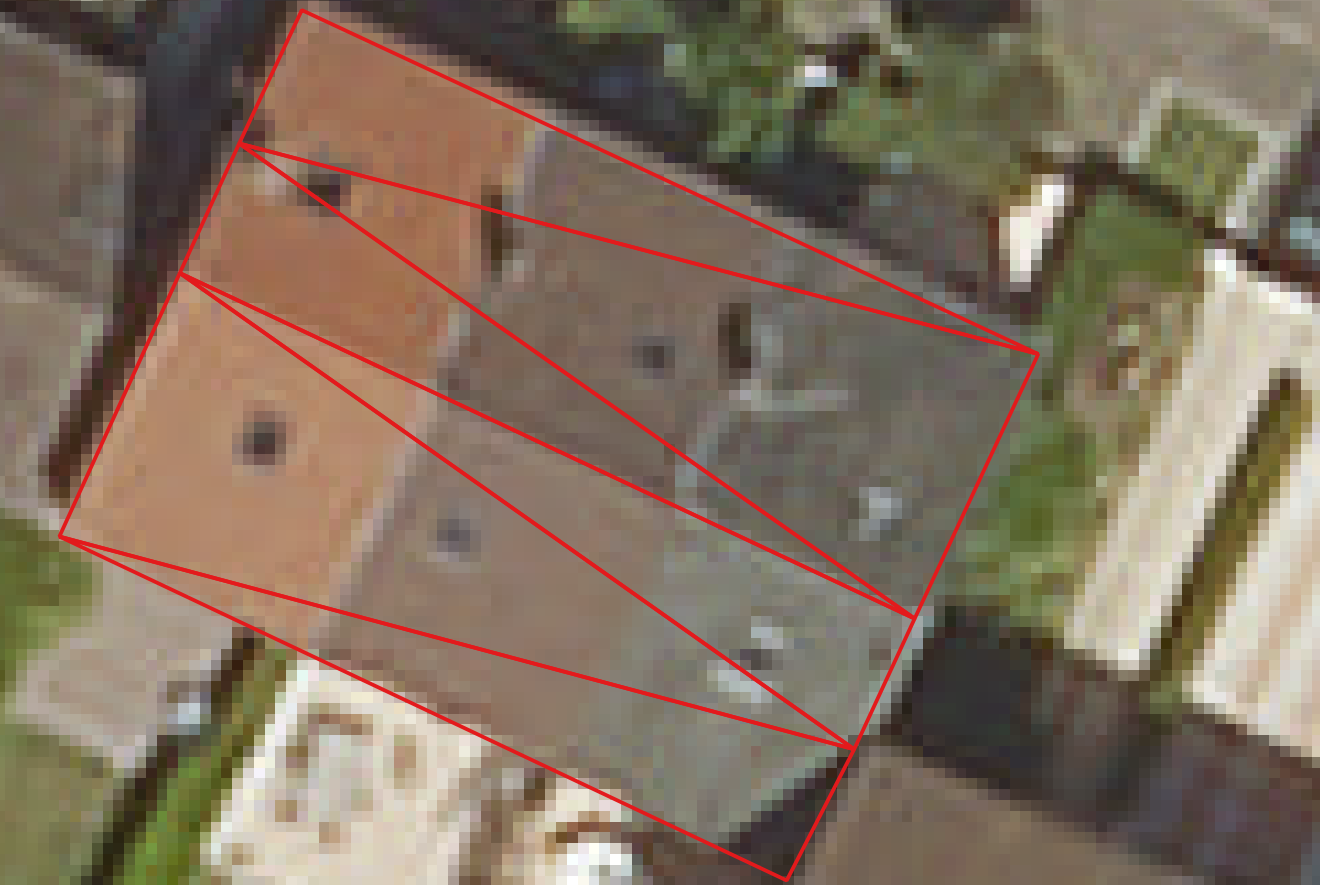
\includegraphics[width=.2\textwidth]{images/errors/building/under_segmentation}}
                    \captionof*{figure}{\tiny Building Under Segmentation.}
                \end{center}
                \begin{center}
                    \fbox{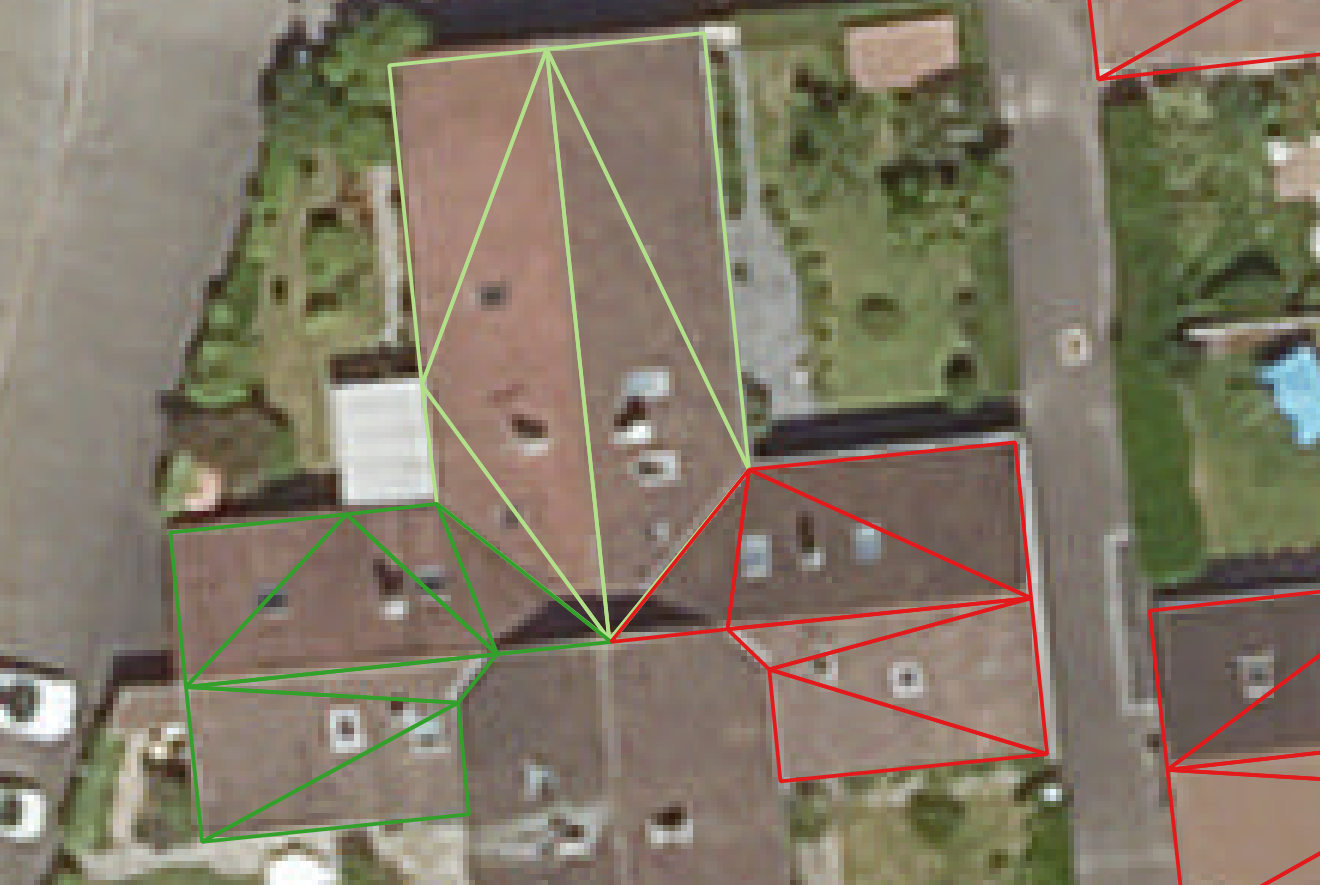
\includegraphics[width=.2\textwidth]{images/errors/building/over_segmentation}}
                    \captionof*{figure}{\tiny Building Over segmentation.}
                \end{center}
                \begin{center}
                    \fbox{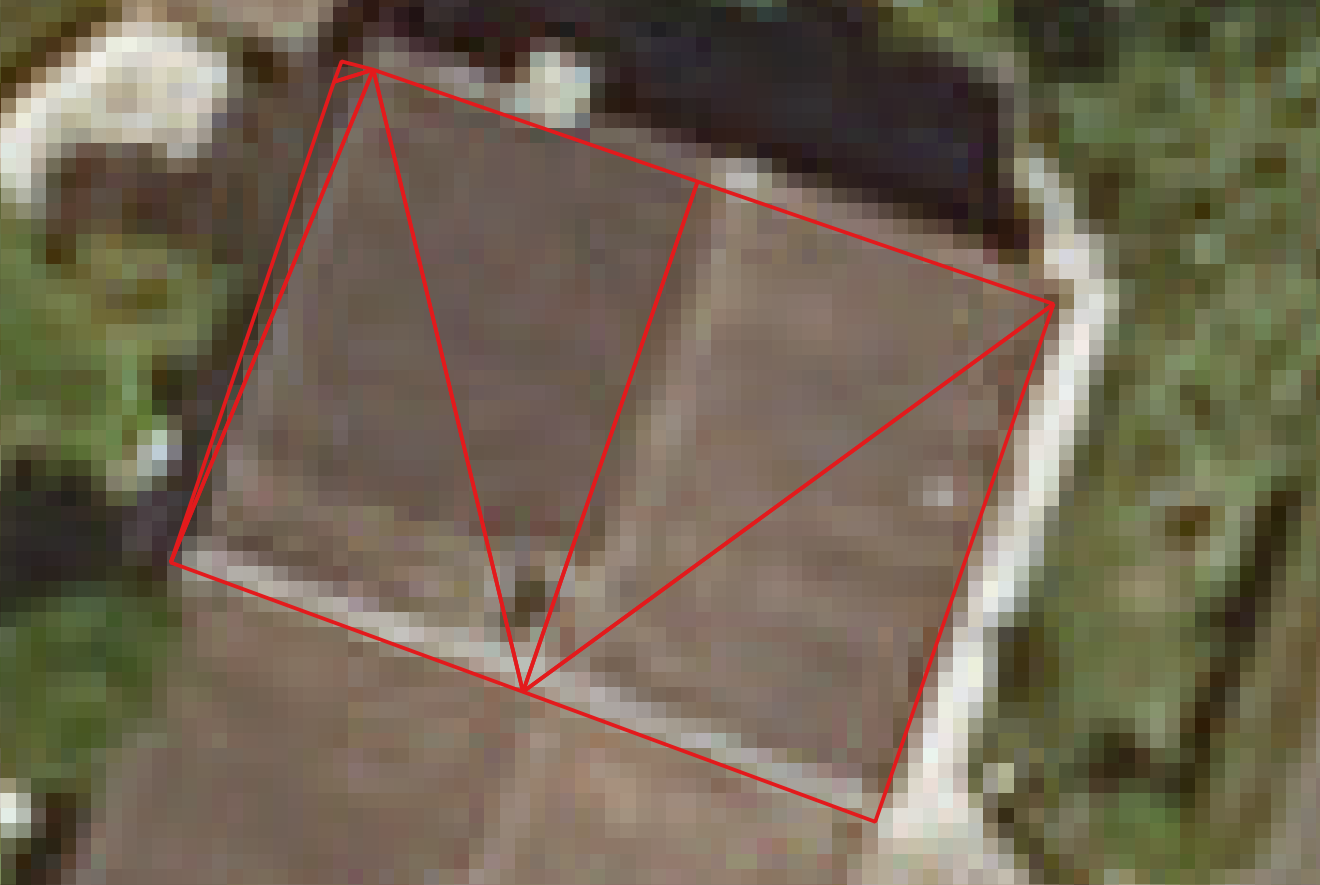
\includegraphics[width=.2\textwidth]{images/errors/building/footprint}}
                    \captionof*{figure}{\tiny Building Footprint Error.}
                \end{center}
                \begin{center}
                    \fbox{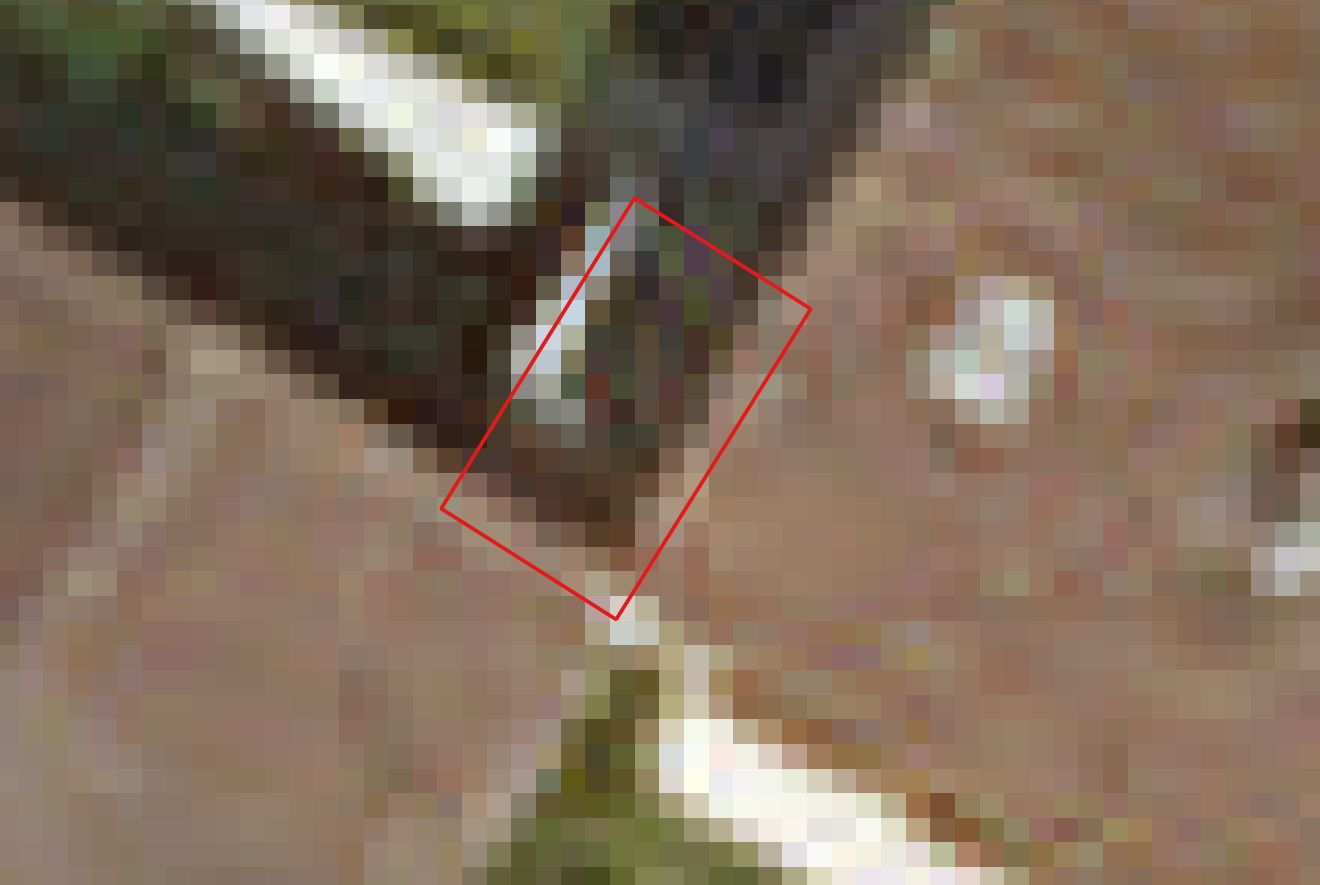
\includegraphics[width=.2\textwidth]{images/errors/building/altimetric}}
                    \captionof*{figure}{\tiny Building Height Error.}
                \end{center}
            \end{multicols}
            \begin{multicols}{4}
                \begin{center}
                    \fbox{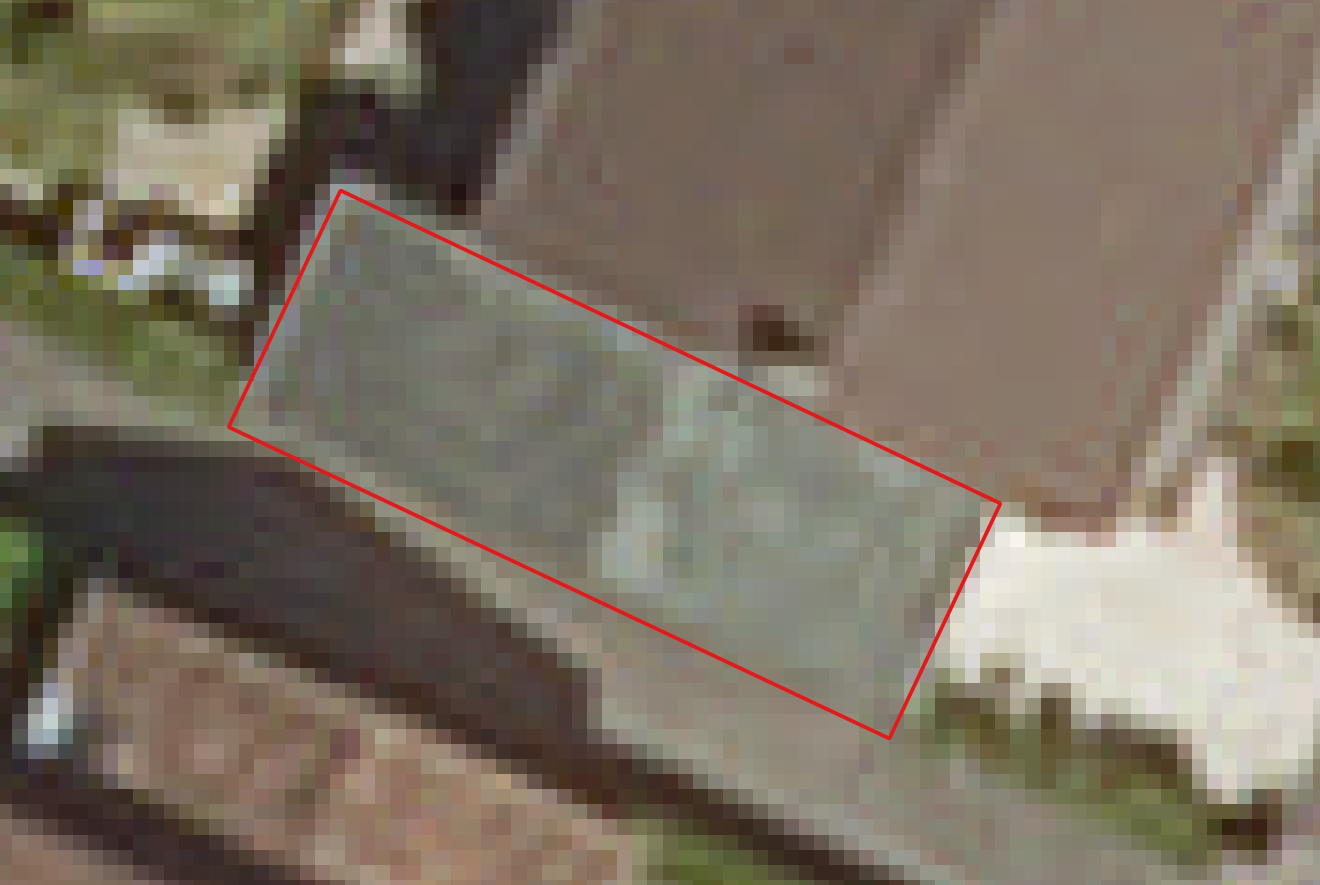
\includegraphics[width=.2\textwidth]{images/errors/facet/under_segmentation}}
                    \captionof*{figure}{\tiny Under Segmentation.}
                \end{center}
                \begin{center}
                    \fbox{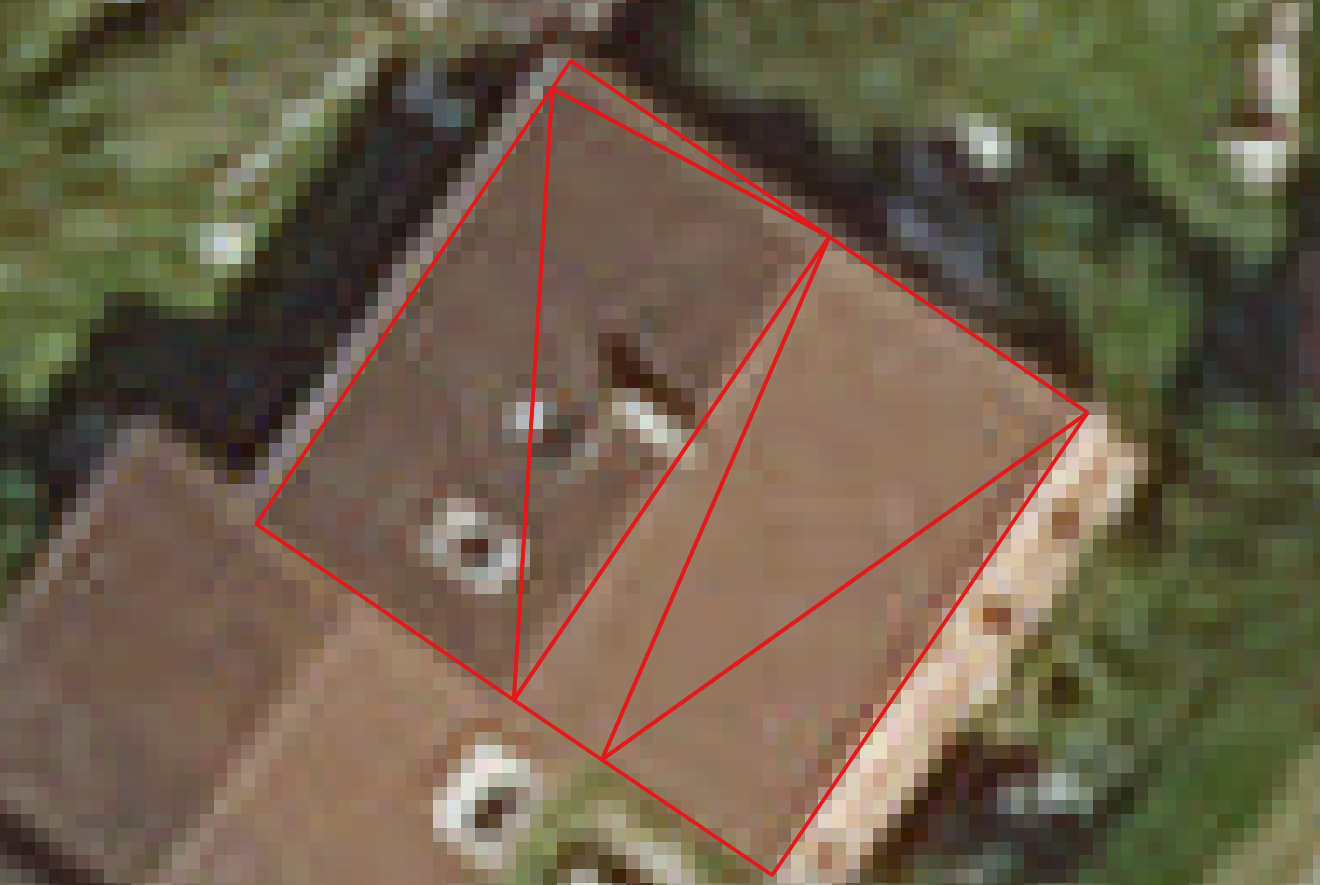
\includegraphics[width=.2\textwidth]{images/errors/facet/over_segmentation}}
                    \captionof*{figure}{\tiny Facet Over Segmentation.}
                \end{center}
                \begin{center}
                    \fbox{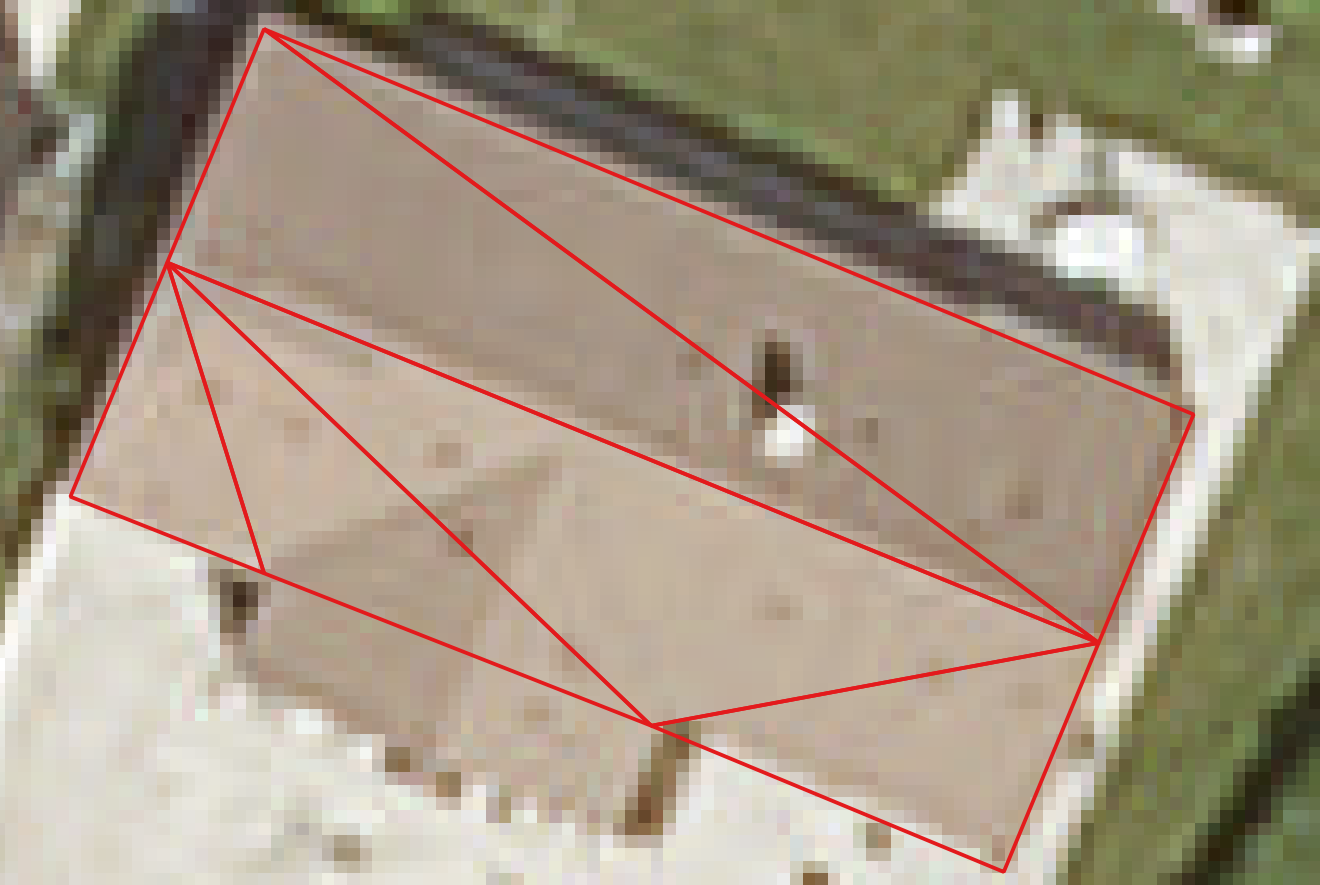
\includegraphics[width=.2\textwidth]{images/errors/facet/mis_segmentation}}
                    \captionof*{figure}{\tiny Facet Imprecise Segmentation.}
                \end{center}
                \begin{center}
                    \fbox{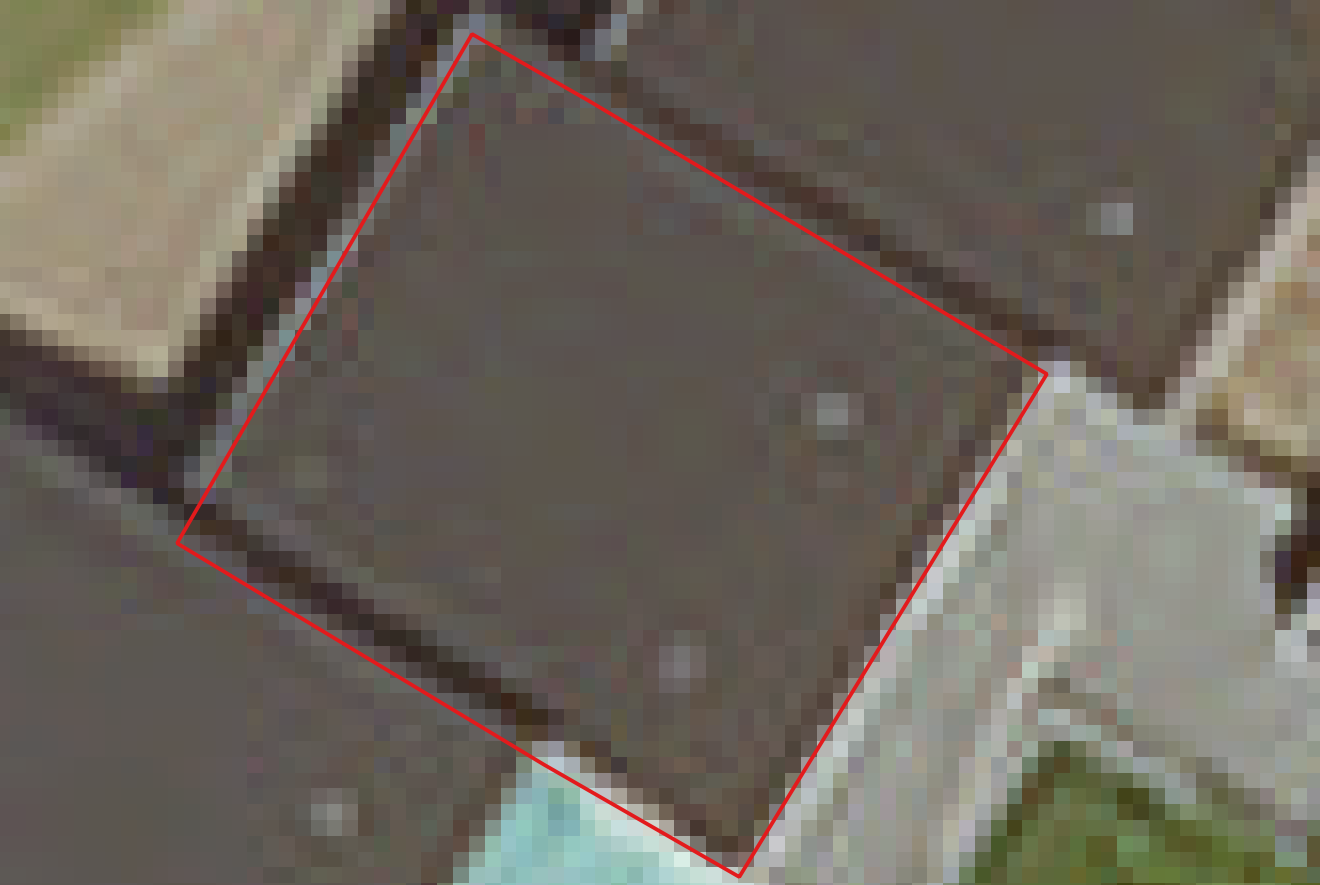
\includegraphics[width=.2\textwidth]{images/errors/facet/slope}}
                    \captionof*{figure}{\tiny Facet Slope Error imprecision.}
                \end{center}
            \end{multicols}
        }

        \StandardBox{results}{column=4, span=2, below=feats, bottomaligned=errors}{Results}{
            {
                \tiny
                \begin{center}
                    \begin{tabular}{x{1.5cm} x{.5cm} x{1cm} x{1cm}}
                        \toprule
                        {\bf Error} & {\bf OA} & {\bf Recall} & {\bf Precision} \\
                        \midrule
                        Building Errors & $0.79$ & $0.35$ & $0.75$ \\
                        \midrule
                        Facet Errors & $0.90$ & $0.96$ & $0.92$ \\
                        \bottomrule
                    \end{tabular}
                    \captionof{subtable}{\tiny\label{tab::finesse2} $finesse = 2$}
                \end{center}
                \begin{center}
                    \begin{tabular}{x{2cm} x{.5cm} x{1cm} x{1cm}}
                        \toprule
                        {\bf Error} & {\bf OA} & {\bf Recall} & {\bf Precision} \\
                        \midrule
                        Buil. Under Seg. & $0.96$ & $0.71$ & $0.88$ \\
                        \midrule
                        Buil. Over Seg. & $0.97$ & $0.06$ & $1.0$ \\
                        \midrule
                        Footprint & $0.89$ & $0.15$ & $1.0$ \\
                        \midrule
                        Height & $0.99$ & $0.0$ & --- \\
                        \midrule
                        \midrule
                        Fac. Under Seg. & $0.92$ & $0.11$ & $0.36$ \\
                        \midrule
                        Fac. Over Seg. & $0.99$ & $.99$ & $0.99$ \\
                        \midrule
                        Fac. Impr. Seg. & $0.92$ & $0.0$ & ---\\
                        \midrule
                        Slope & $0.97$ & $0.07$ & $1.0$\\
                        \bottomrule
                    \end{tabular}
                    \captionof{subtable}{\tiny\label{tab::finesse3}$finesse = 3$}
                \end{center}
            }
            \begin{center}
                Test results for a \textit{non exclusive} qualification with $ LoD = 2 $ using a $10-fold$ classification and all ($4\times4 + 10 + 10 = 36$) features.
            \end{center}
        }

        \ReferencesBox{references}{column=0, span=5, below=errors}{\bf{References}}{
            \setlength{\columnseprule}{0.1pt}
            \begin{multicols}{3}
                \renewcommand{\section}[2]{}
                \bibliographystyle{abbrv}
                \tiny \bibliography{references}
            \end{multicols}
        }

        \InvisibleBox{qr}{column=5, span=1, aligned=references}{}{
            \vspace{-.3cm}
            \begin{center}
                
\includegraphics[width=\textwidth]{qr}
            \end{center}
        }

        \InvisibleBox{event}{column=2, span=2, row=.985}{}{
            \begin{tikzpicture}
                \node[rectangle, minimum width=\textwidth]{
                    \footnotesize{CFPT 2018}
                };
            \end{tikzpicture}
        }
    \end{poster}
\end{document}
